% Options for packages loaded elsewhere
\PassOptionsToPackage{unicode}{hyperref}
\PassOptionsToPackage{hyphens}{url}
%
\documentclass[
]{article}
\usepackage{amsmath,amssymb}
\usepackage{iftex}
\ifPDFTeX
  \usepackage[T1]{fontenc}
  \usepackage[utf8]{inputenc}
  \usepackage{textcomp} % provide euro and other symbols
\else % if luatex or xetex
  \usepackage{unicode-math} % this also loads fontspec
  \defaultfontfeatures{Scale=MatchLowercase}
  \defaultfontfeatures[\rmfamily]{Ligatures=TeX,Scale=1}
\fi
\usepackage{lmodern}
\ifPDFTeX\else
  % xetex/luatex font selection
\fi
% Use upquote if available, for straight quotes in verbatim environments
\IfFileExists{upquote.sty}{\usepackage{upquote}}{}
\IfFileExists{microtype.sty}{% use microtype if available
  \usepackage[]{microtype}
  \UseMicrotypeSet[protrusion]{basicmath} % disable protrusion for tt fonts
}{}
\makeatletter
\@ifundefined{KOMAClassName}{% if non-KOMA class
  \IfFileExists{parskip.sty}{%
    \usepackage{parskip}
  }{% else
    \setlength{\parindent}{0pt}
    \setlength{\parskip}{6pt plus 2pt minus 1pt}}
}{% if KOMA class
  \KOMAoptions{parskip=half}}
\makeatother
\usepackage{xcolor}
\usepackage[margin=1in]{geometry}
\usepackage{color}
\usepackage{fancyvrb}
\newcommand{\VerbBar}{|}
\newcommand{\VERB}{\Verb[commandchars=\\\{\}]}
\DefineVerbatimEnvironment{Highlighting}{Verbatim}{commandchars=\\\{\}}
% Add ',fontsize=\small' for more characters per line
\usepackage{framed}
\definecolor{shadecolor}{RGB}{248,248,248}
\newenvironment{Shaded}{\begin{snugshade}}{\end{snugshade}}
\newcommand{\AlertTok}[1]{\textcolor[rgb]{0.94,0.16,0.16}{#1}}
\newcommand{\AnnotationTok}[1]{\textcolor[rgb]{0.56,0.35,0.01}{\textbf{\textit{#1}}}}
\newcommand{\AttributeTok}[1]{\textcolor[rgb]{0.13,0.29,0.53}{#1}}
\newcommand{\BaseNTok}[1]{\textcolor[rgb]{0.00,0.00,0.81}{#1}}
\newcommand{\BuiltInTok}[1]{#1}
\newcommand{\CharTok}[1]{\textcolor[rgb]{0.31,0.60,0.02}{#1}}
\newcommand{\CommentTok}[1]{\textcolor[rgb]{0.56,0.35,0.01}{\textit{#1}}}
\newcommand{\CommentVarTok}[1]{\textcolor[rgb]{0.56,0.35,0.01}{\textbf{\textit{#1}}}}
\newcommand{\ConstantTok}[1]{\textcolor[rgb]{0.56,0.35,0.01}{#1}}
\newcommand{\ControlFlowTok}[1]{\textcolor[rgb]{0.13,0.29,0.53}{\textbf{#1}}}
\newcommand{\DataTypeTok}[1]{\textcolor[rgb]{0.13,0.29,0.53}{#1}}
\newcommand{\DecValTok}[1]{\textcolor[rgb]{0.00,0.00,0.81}{#1}}
\newcommand{\DocumentationTok}[1]{\textcolor[rgb]{0.56,0.35,0.01}{\textbf{\textit{#1}}}}
\newcommand{\ErrorTok}[1]{\textcolor[rgb]{0.64,0.00,0.00}{\textbf{#1}}}
\newcommand{\ExtensionTok}[1]{#1}
\newcommand{\FloatTok}[1]{\textcolor[rgb]{0.00,0.00,0.81}{#1}}
\newcommand{\FunctionTok}[1]{\textcolor[rgb]{0.13,0.29,0.53}{\textbf{#1}}}
\newcommand{\ImportTok}[1]{#1}
\newcommand{\InformationTok}[1]{\textcolor[rgb]{0.56,0.35,0.01}{\textbf{\textit{#1}}}}
\newcommand{\KeywordTok}[1]{\textcolor[rgb]{0.13,0.29,0.53}{\textbf{#1}}}
\newcommand{\NormalTok}[1]{#1}
\newcommand{\OperatorTok}[1]{\textcolor[rgb]{0.81,0.36,0.00}{\textbf{#1}}}
\newcommand{\OtherTok}[1]{\textcolor[rgb]{0.56,0.35,0.01}{#1}}
\newcommand{\PreprocessorTok}[1]{\textcolor[rgb]{0.56,0.35,0.01}{\textit{#1}}}
\newcommand{\RegionMarkerTok}[1]{#1}
\newcommand{\SpecialCharTok}[1]{\textcolor[rgb]{0.81,0.36,0.00}{\textbf{#1}}}
\newcommand{\SpecialStringTok}[1]{\textcolor[rgb]{0.31,0.60,0.02}{#1}}
\newcommand{\StringTok}[1]{\textcolor[rgb]{0.31,0.60,0.02}{#1}}
\newcommand{\VariableTok}[1]{\textcolor[rgb]{0.00,0.00,0.00}{#1}}
\newcommand{\VerbatimStringTok}[1]{\textcolor[rgb]{0.31,0.60,0.02}{#1}}
\newcommand{\WarningTok}[1]{\textcolor[rgb]{0.56,0.35,0.01}{\textbf{\textit{#1}}}}
\usepackage{graphicx}
\makeatletter
\def\maxwidth{\ifdim\Gin@nat@width>\linewidth\linewidth\else\Gin@nat@width\fi}
\def\maxheight{\ifdim\Gin@nat@height>\textheight\textheight\else\Gin@nat@height\fi}
\makeatother
% Scale images if necessary, so that they will not overflow the page
% margins by default, and it is still possible to overwrite the defaults
% using explicit options in \includegraphics[width, height, ...]{}
\setkeys{Gin}{width=\maxwidth,height=\maxheight,keepaspectratio}
% Set default figure placement to htbp
\makeatletter
\def\fps@figure{htbp}
\makeatother
\setlength{\emergencystretch}{3em} % prevent overfull lines
\providecommand{\tightlist}{%
  \setlength{\itemsep}{0pt}\setlength{\parskip}{0pt}}
\setcounter{secnumdepth}{-\maxdimen} % remove section numbering
\ifLuaTeX
  \usepackage{selnolig}  % disable illegal ligatures
\fi
\IfFileExists{bookmark.sty}{\usepackage{bookmark}}{\usepackage{hyperref}}
\IfFileExists{xurl.sty}{\usepackage{xurl}}{} % add URL line breaks if available
\urlstyle{same}
\hypersetup{
  pdftitle={S optimize bias, all samples, cohort1},
  pdfauthor={Sean Maden},
  hidelinks,
  pdfcreator={LaTeX via pandoc}}

\title{S optimize bias, all samples, cohort1}
\author{Sean Maden}
\date{2023-08-08}

\begin{document}
\maketitle

\hypertarget{key-experiment-notes}{%
\section{Key experiment notes}\label{key-experiment-notes}}

This experiment utilizes the same Y, Z, P definition scheme as the
pseudobulk experiments 02 scripts.

\hypertarget{load-results}{%
\section{load results}\label{load-results}}

\begin{Shaded}
\begin{Highlighting}[]
\CommentTok{\# load the dataset}
\FunctionTok{setwd}\NormalTok{(}\StringTok{".."}\NormalTok{)}
\FunctionTok{setwd}\NormalTok{(}\StringTok{".."}\NormalTok{)}
\NormalTok{load.filename }\OtherTok{\textless{}{-}} \StringTok{"df{-}result\_s{-}opt{-}bias\_cohort1.rda"}
\NormalTok{load.path }\OtherTok{\textless{}{-}} \FunctionTok{file.path}\NormalTok{(}\StringTok{"outputs"}\NormalTok{, }\StringTok{"11\_soptimize{-}pbfit{-}bias\_dlpfc{-}cohort1"}\NormalTok{, load.filename)}
\NormalTok{df.res }\OtherTok{\textless{}{-}} \FunctionTok{get}\NormalTok{(}\FunctionTok{load}\NormalTok{(load.path))}
\NormalTok{df.res}\SpecialCharTok{$}\NormalTok{abs.bias.neuron }\OtherTok{\textless{}{-}} \FunctionTok{abs}\NormalTok{(df.res}\SpecialCharTok{$}\NormalTok{bias.neuron.true.pred)}

\CommentTok{\# do postprocessing on the dataset}
\CommentTok{\# rename abs bias colname to error}
\NormalTok{colnames.filter }\OtherTok{\textless{}{-}} \FunctionTok{colnames}\NormalTok{(df.res)}\SpecialCharTok{==}\StringTok{"abs.bias.neuron"}
\FunctionTok{colnames}\NormalTok{(df.res)[colnames.filter] }\OtherTok{\textless{}{-}} \StringTok{"error.neuron"}
\CommentTok{\# add group labels}
\NormalTok{df.res}\SpecialCharTok{$}\NormalTok{glial.group.label }\OtherTok{\textless{}{-}} \FunctionTok{as.character}\NormalTok{(df.res}\SpecialCharTok{$}\NormalTok{glial)}
\NormalTok{df.res}\SpecialCharTok{$}\NormalTok{neuron.group.label }\OtherTok{\textless{}{-}} \FunctionTok{as.character}\NormalTok{(df.res}\SpecialCharTok{$}\NormalTok{neuron)}
\CommentTok{\# append highlight values}
\NormalTok{df.res}\SpecialCharTok{$}\NormalTok{minimum.error }\OtherTok{\textless{}{-}}\NormalTok{ df.res}\SpecialCharTok{$}\NormalTok{error.neuron}\SpecialCharTok{==}\FunctionTok{min}\NormalTok{(df.res}\SpecialCharTok{$}\NormalTok{error.neuron)}
\NormalTok{df.res}\SpecialCharTok{$}\NormalTok{maximum.error }\OtherTok{\textless{}{-}}\NormalTok{ df.res}\SpecialCharTok{$}\NormalTok{error.neuron}\SpecialCharTok{==}\FunctionTok{max}\NormalTok{(df.res}\SpecialCharTok{$}\NormalTok{error.neuron)}
\CommentTok{\# assign deciles}
\NormalTok{quant }\OtherTok{\textless{}{-}} \FunctionTok{quantile}\NormalTok{(df.res}\SpecialCharTok{$}\NormalTok{error.neuron, }\FunctionTok{seq}\NormalTok{(}\DecValTok{0}\NormalTok{,}\DecValTok{1}\NormalTok{,}\FloatTok{0.1}\NormalTok{))}
\NormalTok{df.res}\SpecialCharTok{$}\NormalTok{lowest.decile.error }\OtherTok{\textless{}{-}}\NormalTok{ df.res}\SpecialCharTok{$}\NormalTok{error.neuron }\SpecialCharTok{\textless{}=}\NormalTok{ quant[}\DecValTok{2}\NormalTok{]}
\NormalTok{df.res}\SpecialCharTok{$}\NormalTok{highest.decile.error }\OtherTok{\textless{}{-}}\NormalTok{ df.res}\SpecialCharTok{$}\NormalTok{error.neuron}\SpecialCharTok{\textgreater{}=}\NormalTok{quant[}\DecValTok{10}\NormalTok{]}

\CommentTok{\# plot params}
\CommentTok{\# highlight colors}
\NormalTok{highlight.color.low }\OtherTok{\textless{}{-}} \StringTok{"red"}
\NormalTok{highlight.color.high }\OtherTok{\textless{}{-}} \StringTok{"blue"}
\NormalTok{highlight.color.background }\OtherTok{\textless{}{-}} \StringTok{"gray"}
\end{Highlighting}
\end{Shaded}

\hypertarget{plot-results-summaries}{%
\section{Plot results summaries}\label{plot-results-summaries}}

Heatmap of k2 scale factors (field axes) by error (gradient).

\begin{Shaded}
\begin{Highlighting}[]
\FunctionTok{ggplot}\NormalTok{(df.res, }\FunctionTok{aes}\NormalTok{(}\AttributeTok{x =}\NormalTok{ neuron, }\AttributeTok{y =}\NormalTok{ glial)) }\SpecialCharTok{+} \FunctionTok{theme\_bw}\NormalTok{() }\SpecialCharTok{+}
  \FunctionTok{geom\_raster}\NormalTok{(}\FunctionTok{aes}\NormalTok{(}\AttributeTok{fill =}\NormalTok{ error.neuron)) }\SpecialCharTok{+}
  \FunctionTok{scale\_fill\_gradientn}\NormalTok{(}\AttributeTok{colours =} \FunctionTok{rainbow}\NormalTok{(}\DecValTok{5}\NormalTok{)) }\SpecialCharTok{+} \FunctionTok{facet\_wrap}\NormalTok{(}\SpecialCharTok{\textasciitilde{}}\NormalTok{sample.id) }\SpecialCharTok{+}
  \FunctionTok{geom\_hline}\NormalTok{(}\AttributeTok{yintercept =} \DecValTok{3}\NormalTok{) }\SpecialCharTok{+} \FunctionTok{geom\_vline}\NormalTok{(}\AttributeTok{xintercept =} \DecValTok{10}\NormalTok{) }\SpecialCharTok{+}
  \FunctionTok{geom\_abline}\NormalTok{(}\AttributeTok{slope =} \DecValTok{1}\NormalTok{, }\AttributeTok{intercept =} \DecValTok{0}\NormalTok{)}
\end{Highlighting}
\end{Shaded}

\includegraphics{pb-byblock_sopt-bias-error_k2-cohort1_files/figure-latex/unnamed-chunk-2-1.pdf}

Scatterplots of K2\_1 by K2\_1 bias, color by block ID.

\begin{Shaded}
\begin{Highlighting}[]
\CommentTok{\# neuron}
\FunctionTok{ggplot}\NormalTok{(df.res, }\FunctionTok{aes}\NormalTok{(}\AttributeTok{x =}\NormalTok{ neuron, }\AttributeTok{y =}\NormalTok{ bias.neuron.true.pred, }\AttributeTok{color =}\NormalTok{ sample.id)) }\SpecialCharTok{+} 
  \FunctionTok{geom\_point}\NormalTok{(}\AttributeTok{alpha =} \FloatTok{0.2}\NormalTok{) }\SpecialCharTok{+} \FunctionTok{theme\_bw}\NormalTok{() }\SpecialCharTok{+} \FunctionTok{facet\_wrap}\NormalTok{(}\SpecialCharTok{\textasciitilde{}}\NormalTok{sample.id) }\SpecialCharTok{+} \FunctionTok{geom\_hline}\NormalTok{(}\AttributeTok{yintercept =} \DecValTok{0}\NormalTok{) }\SpecialCharTok{+}
  \FunctionTok{ggtitle}\NormalTok{(}\StringTok{"Neuron"}\NormalTok{)}
\end{Highlighting}
\end{Shaded}

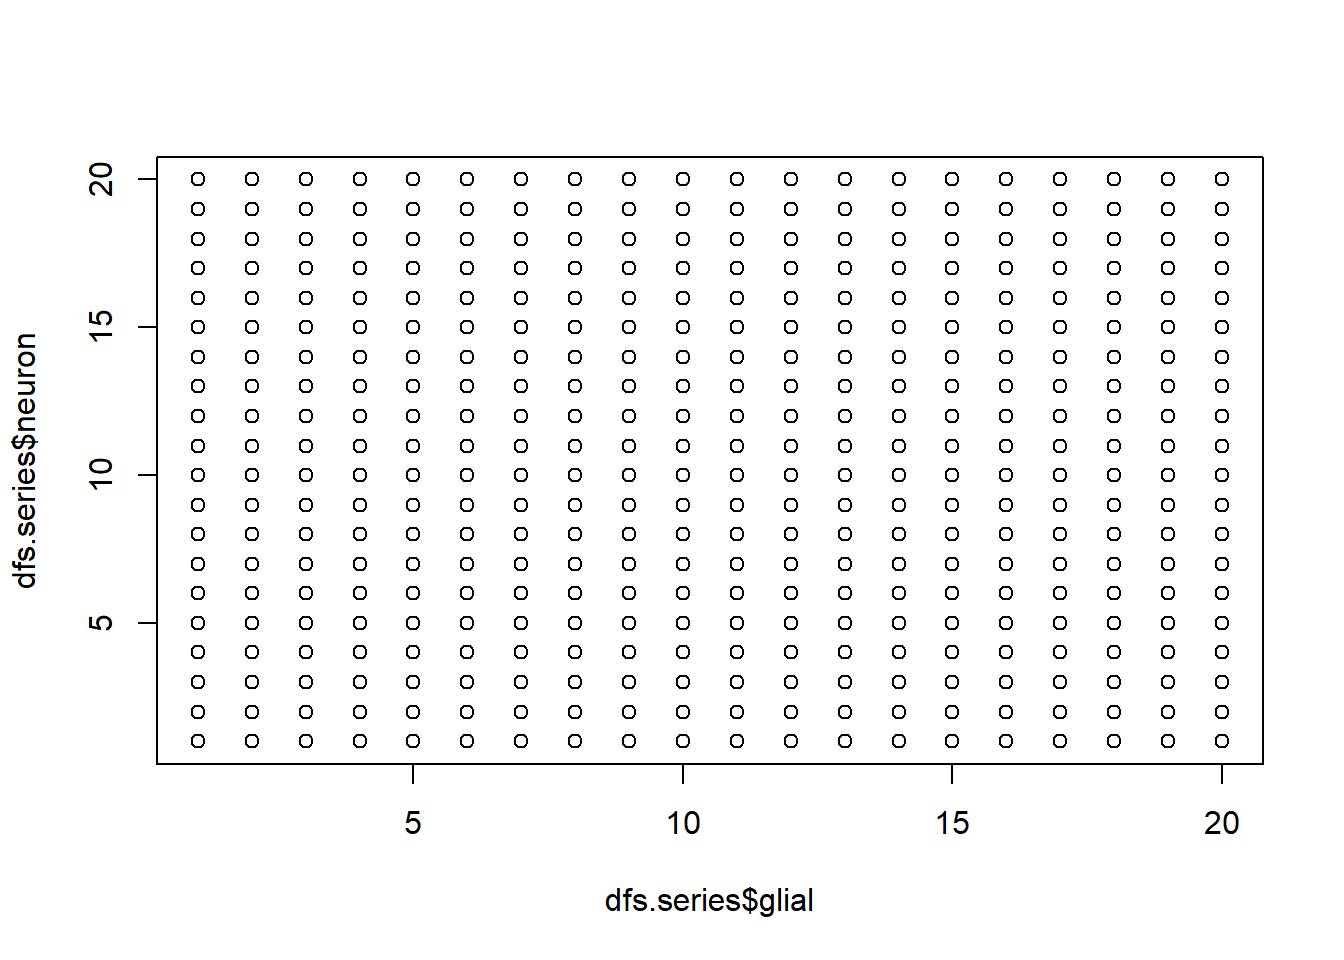
\includegraphics{pb-byblock_sopt-bias-error_k2-cohort1_files/figure-latex/unnamed-chunk-3-1.pdf}

\begin{Shaded}
\begin{Highlighting}[]
\CommentTok{\# glial}
\FunctionTok{ggplot}\NormalTok{(df.res, }\FunctionTok{aes}\NormalTok{(}\AttributeTok{x =}\NormalTok{ glial, }\AttributeTok{y =}\NormalTok{ bias.glial.true.pred, }\AttributeTok{color =}\NormalTok{ sample.id)) }\SpecialCharTok{+} 
  \FunctionTok{geom\_point}\NormalTok{(}\AttributeTok{alpha =} \FloatTok{0.2}\NormalTok{) }\SpecialCharTok{+} \FunctionTok{theme\_bw}\NormalTok{() }\SpecialCharTok{+} \FunctionTok{facet\_wrap}\NormalTok{(}\SpecialCharTok{\textasciitilde{}}\NormalTok{sample.id) }\SpecialCharTok{+} \FunctionTok{geom\_hline}\NormalTok{(}\AttributeTok{yintercept =} \DecValTok{0}\NormalTok{) }\SpecialCharTok{+}
  \FunctionTok{ggtitle}\NormalTok{(}\StringTok{"Glial"}\NormalTok{)}
\end{Highlighting}
\end{Shaded}

\includegraphics{pb-byblock_sopt-bias-error_k2-cohort1_files/figure-latex/unnamed-chunk-3-2.pdf}

Line plots of K2\_1 by K2\_1 bias, group by K2\_2 factor, facet by block
ID.

\begin{Shaded}
\begin{Highlighting}[]
\CommentTok{\# neuron}
\FunctionTok{ggplot}\NormalTok{(df.res, }\FunctionTok{aes}\NormalTok{(}\AttributeTok{x =}\NormalTok{ neuron, }\AttributeTok{y =}\NormalTok{ bias.neuron.true.pred, }
                   \AttributeTok{group =}\NormalTok{ glial.group.label, }\AttributeTok{color =}\NormalTok{ glial.group.label)) }\SpecialCharTok{+} 
  \FunctionTok{geom\_line}\NormalTok{() }\SpecialCharTok{+} \FunctionTok{theme\_bw}\NormalTok{() }\SpecialCharTok{+} \FunctionTok{facet\_wrap}\NormalTok{(}\SpecialCharTok{\textasciitilde{}}\NormalTok{sample.id) }\SpecialCharTok{+} \FunctionTok{geom\_hline}\NormalTok{(}\AttributeTok{yintercept =} \DecValTok{0}\NormalTok{) }\SpecialCharTok{+}
  \FunctionTok{ggtitle}\NormalTok{(}\StringTok{"Neuron"}\NormalTok{)}
\end{Highlighting}
\end{Shaded}

\includegraphics{pb-byblock_sopt-bias-error_k2-cohort1_files/figure-latex/unnamed-chunk-4-1.pdf}

\begin{Shaded}
\begin{Highlighting}[]
\CommentTok{\# glial}
\FunctionTok{ggplot}\NormalTok{(df.res, }\FunctionTok{aes}\NormalTok{(}\AttributeTok{x =}\NormalTok{ glial, }\AttributeTok{y =}\NormalTok{ bias.glial.true.pred, }
                   \AttributeTok{group =}\NormalTok{ neuron.group.label, }\AttributeTok{color =}\NormalTok{ neuron.group.label)) }\SpecialCharTok{+} 
  \FunctionTok{geom\_line}\NormalTok{() }\SpecialCharTok{+} \FunctionTok{theme\_bw}\NormalTok{() }\SpecialCharTok{+} \FunctionTok{facet\_wrap}\NormalTok{(}\SpecialCharTok{\textasciitilde{}}\NormalTok{sample.id) }\SpecialCharTok{+} \FunctionTok{geom\_hline}\NormalTok{(}\AttributeTok{yintercept =} \DecValTok{0}\NormalTok{) }\SpecialCharTok{+}
  \FunctionTok{ggtitle}\NormalTok{(}\StringTok{"Glial"}\NormalTok{)}
\end{Highlighting}
\end{Shaded}

\includegraphics{pb-byblock_sopt-bias-error_k2-cohort1_files/figure-latex/unnamed-chunk-4-2.pdf}

Scatterplots of K2\_1 by K2\_1 bias, color by K2\_2 cell size --
discrete.

\begin{Shaded}
\begin{Highlighting}[]
\CommentTok{\# neuron}
\FunctionTok{ggplot}\NormalTok{(df.res, }\FunctionTok{aes}\NormalTok{(}\AttributeTok{x =}\NormalTok{ neuron, }\AttributeTok{y =}\NormalTok{ bias.neuron.true.pred, }\AttributeTok{color =}\NormalTok{ glial.group.label)) }\SpecialCharTok{+} 
  \FunctionTok{geom\_point}\NormalTok{(}\AttributeTok{alpha =} \FloatTok{0.2}\NormalTok{) }\SpecialCharTok{+} \FunctionTok{theme\_bw}\NormalTok{() }\SpecialCharTok{+} \FunctionTok{facet\_wrap}\NormalTok{(}\SpecialCharTok{\textasciitilde{}}\NormalTok{sample.id) }\SpecialCharTok{+} \FunctionTok{geom\_hline}\NormalTok{(}\AttributeTok{yintercept =} \DecValTok{0}\NormalTok{) }\SpecialCharTok{+}
  \FunctionTok{ggtitle}\NormalTok{(}\StringTok{"Neuron"}\NormalTok{)}
\end{Highlighting}
\end{Shaded}

\includegraphics{pb-byblock_sopt-bias-error_k2-cohort1_files/figure-latex/unnamed-chunk-5-1.pdf}

\begin{Shaded}
\begin{Highlighting}[]
\CommentTok{\# glial}
\FunctionTok{ggplot}\NormalTok{(df.res, }\FunctionTok{aes}\NormalTok{(}\AttributeTok{x =}\NormalTok{ glial, }\AttributeTok{y =}\NormalTok{ bias.glial.true.pred, }\AttributeTok{color =}\NormalTok{ neuron.group.label)) }\SpecialCharTok{+} 
  \FunctionTok{geom\_point}\NormalTok{(}\AttributeTok{alpha =} \FloatTok{0.2}\NormalTok{) }\SpecialCharTok{+} \FunctionTok{theme\_bw}\NormalTok{() }\SpecialCharTok{+} \FunctionTok{facet\_wrap}\NormalTok{(}\SpecialCharTok{\textasciitilde{}}\NormalTok{sample.id) }\SpecialCharTok{+} \FunctionTok{geom\_hline}\NormalTok{(}\AttributeTok{yintercept =} \DecValTok{0}\NormalTok{) }\SpecialCharTok{+}
  \FunctionTok{ggtitle}\NormalTok{(}\StringTok{"Glial"}\NormalTok{)}
\end{Highlighting}
\end{Shaded}

\includegraphics{pb-byblock_sopt-bias-error_k2-cohort1_files/figure-latex/unnamed-chunk-5-2.pdf}

Scatterplots of K2\_1 by K2\_1 bias, color by K2\_2 cell size --
continuous.

\begin{Shaded}
\begin{Highlighting}[]
\CommentTok{\# neuron}
\FunctionTok{ggplot}\NormalTok{(df.res, }\FunctionTok{aes}\NormalTok{(}\AttributeTok{x =}\NormalTok{ neuron, }\AttributeTok{y =}\NormalTok{ bias.neuron.true.pred, }\AttributeTok{color =}\NormalTok{ glial)) }\SpecialCharTok{+} 
  \FunctionTok{geom\_point}\NormalTok{(}\AttributeTok{alpha =} \FloatTok{0.2}\NormalTok{) }\SpecialCharTok{+} \FunctionTok{theme\_bw}\NormalTok{() }\SpecialCharTok{+} \FunctionTok{facet\_wrap}\NormalTok{(}\SpecialCharTok{\textasciitilde{}}\NormalTok{sample.id) }\SpecialCharTok{+} \FunctionTok{geom\_hline}\NormalTok{(}\AttributeTok{yintercept =} \DecValTok{0}\NormalTok{) }\SpecialCharTok{+}
  \FunctionTok{ggtitle}\NormalTok{(}\StringTok{"Neuron"}\NormalTok{)}
\end{Highlighting}
\end{Shaded}

\includegraphics{pb-byblock_sopt-bias-error_k2-cohort1_files/figure-latex/unnamed-chunk-6-1.pdf}

\begin{Shaded}
\begin{Highlighting}[]
\CommentTok{\# glial}
\FunctionTok{ggplot}\NormalTok{(df.res, }\FunctionTok{aes}\NormalTok{(}\AttributeTok{x =}\NormalTok{ glial, }\AttributeTok{y =}\NormalTok{ bias.glial.true.pred, }\AttributeTok{color =}\NormalTok{ neuron)) }\SpecialCharTok{+} 
  \FunctionTok{geom\_point}\NormalTok{(}\AttributeTok{alpha =} \FloatTok{0.2}\NormalTok{) }\SpecialCharTok{+} \FunctionTok{theme\_bw}\NormalTok{() }\SpecialCharTok{+} \FunctionTok{facet\_wrap}\NormalTok{(}\SpecialCharTok{\textasciitilde{}}\NormalTok{sample.id) }\SpecialCharTok{+} \FunctionTok{geom\_hline}\NormalTok{(}\AttributeTok{yintercept =} \DecValTok{0}\NormalTok{) }\SpecialCharTok{+}
  \FunctionTok{ggtitle}\NormalTok{(}\StringTok{"Glial"}\NormalTok{)}
\end{Highlighting}
\end{Shaded}

\includegraphics{pb-byblock_sopt-bias-error_k2-cohort1_files/figure-latex/unnamed-chunk-6-2.pdf}

\hypertarget{plot-error-highlights}{%
\section{Plot error highlights}\label{plot-error-highlights}}

Highlight lowest and highest error values.

Highlight minimum and lowest decile error.

\begin{Shaded}
\begin{Highlighting}[]
\CommentTok{\# minimum}
\FunctionTok{ggplot}\NormalTok{(df.res, }\FunctionTok{aes}\NormalTok{(}\AttributeTok{x =}\NormalTok{ neuron, }\AttributeTok{y =}\NormalTok{ glial, }\AttributeTok{color =}\NormalTok{ minimum.error)) }\SpecialCharTok{+} 
  \FunctionTok{geom\_point}\NormalTok{() }\SpecialCharTok{+} \FunctionTok{scale\_color\_manual}\NormalTok{(}\AttributeTok{values =} \FunctionTok{c}\NormalTok{(}\StringTok{"TRUE"} \OtherTok{=}\NormalTok{ highlight.color.low, }\StringTok{"FALSE"} \OtherTok{=}\NormalTok{ highlight.color.background)) }\SpecialCharTok{+}
  \FunctionTok{facet\_wrap}\NormalTok{(}\SpecialCharTok{\textasciitilde{}}\NormalTok{sample.id) }\SpecialCharTok{+} 
  \FunctionTok{geom\_abline}\NormalTok{(}\AttributeTok{slope =} \DecValTok{1}\NormalTok{, }\AttributeTok{intercept =} \DecValTok{0}\NormalTok{) }\SpecialCharTok{+} \FunctionTok{geom\_hline}\NormalTok{(}\AttributeTok{yintercept =} \DecValTok{3}\NormalTok{) }\SpecialCharTok{+} \FunctionTok{geom\_vline}\NormalTok{(}\AttributeTok{xintercept =} \DecValTok{10}\NormalTok{)}
\end{Highlighting}
\end{Shaded}

\includegraphics{pb-byblock_sopt-bias-error_k2-cohort1_files/figure-latex/unnamed-chunk-7-1.pdf}

\begin{Shaded}
\begin{Highlighting}[]
\CommentTok{\# lowest decile}
\FunctionTok{ggplot}\NormalTok{(df.res, }\FunctionTok{aes}\NormalTok{(}\AttributeTok{x =}\NormalTok{ neuron, }\AttributeTok{y =}\NormalTok{ glial, }\AttributeTok{color =}\NormalTok{ lowest.decile.error)) }\SpecialCharTok{+} 
  \FunctionTok{geom\_point}\NormalTok{() }\SpecialCharTok{+} \FunctionTok{scale\_color\_manual}\NormalTok{(}\AttributeTok{values =} \FunctionTok{c}\NormalTok{(}\StringTok{"TRUE"} \OtherTok{=}\NormalTok{ highlight.color.low, }\StringTok{"FALSE"} \OtherTok{=}\NormalTok{ highlight.color.background)) }\SpecialCharTok{+}
  \FunctionTok{facet\_wrap}\NormalTok{(}\SpecialCharTok{\textasciitilde{}}\NormalTok{sample.id) }\SpecialCharTok{+}
  \FunctionTok{geom\_abline}\NormalTok{(}\AttributeTok{slope =} \DecValTok{1}\NormalTok{, }\AttributeTok{intercept =} \DecValTok{0}\NormalTok{) }\SpecialCharTok{+} \FunctionTok{geom\_hline}\NormalTok{(}\AttributeTok{yintercept =} \DecValTok{3}\NormalTok{) }\SpecialCharTok{+} \FunctionTok{geom\_vline}\NormalTok{(}\AttributeTok{xintercept =} \DecValTok{10}\NormalTok{)}
\end{Highlighting}
\end{Shaded}

\includegraphics{pb-byblock_sopt-bias-error_k2-cohort1_files/figure-latex/unnamed-chunk-7-2.pdf}

Highlight maximum and highest decile error.

\begin{Shaded}
\begin{Highlighting}[]
\CommentTok{\# maximum}
\FunctionTok{ggplot}\NormalTok{(df.res, }\FunctionTok{aes}\NormalTok{(}\AttributeTok{x =}\NormalTok{ neuron, }\AttributeTok{y =}\NormalTok{ glial, }\AttributeTok{color =}\NormalTok{ maximum.error)) }\SpecialCharTok{+} \FunctionTok{geom\_point}\NormalTok{() }\SpecialCharTok{+} 
  \FunctionTok{scale\_color\_manual}\NormalTok{(}\AttributeTok{values =} \FunctionTok{c}\NormalTok{(}\StringTok{"TRUE"} \OtherTok{=}\NormalTok{ highlight.color.high, }\StringTok{"FALSE"} \OtherTok{=}\NormalTok{ highlight.color.background)) }\SpecialCharTok{+}
  \FunctionTok{facet\_wrap}\NormalTok{(}\SpecialCharTok{\textasciitilde{}}\NormalTok{sample.id) }\SpecialCharTok{+}
  \FunctionTok{geom\_abline}\NormalTok{(}\AttributeTok{slope =} \DecValTok{1}\NormalTok{, }\AttributeTok{intercept =} \DecValTok{0}\NormalTok{) }\SpecialCharTok{+} \FunctionTok{geom\_hline}\NormalTok{(}\AttributeTok{yintercept =} \DecValTok{3}\NormalTok{) }\SpecialCharTok{+} \FunctionTok{geom\_vline}\NormalTok{(}\AttributeTok{xintercept =} \DecValTok{10}\NormalTok{)}
\end{Highlighting}
\end{Shaded}

\includegraphics{pb-byblock_sopt-bias-error_k2-cohort1_files/figure-latex/unnamed-chunk-8-1.pdf}

\begin{Shaded}
\begin{Highlighting}[]
\CommentTok{\# maximum decile}
\FunctionTok{ggplot}\NormalTok{(df.res, }\FunctionTok{aes}\NormalTok{(}\AttributeTok{x =}\NormalTok{ neuron, }\AttributeTok{y =}\NormalTok{ glial, }\AttributeTok{color =}\NormalTok{ highest.decile.error)) }\SpecialCharTok{+} \FunctionTok{geom\_point}\NormalTok{() }\SpecialCharTok{+} 
  \FunctionTok{scale\_color\_manual}\NormalTok{(}\AttributeTok{values =} \FunctionTok{c}\NormalTok{(}\StringTok{"TRUE"} \OtherTok{=}\NormalTok{ highlight.color.high, }\StringTok{"FALSE"} \OtherTok{=}\NormalTok{ highlight.color.background)) }\SpecialCharTok{+}
  \FunctionTok{facet\_wrap}\NormalTok{(}\SpecialCharTok{\textasciitilde{}}\NormalTok{sample.id) }\SpecialCharTok{+}
  \FunctionTok{geom\_abline}\NormalTok{(}\AttributeTok{slope =} \DecValTok{1}\NormalTok{, }\AttributeTok{intercept =} \DecValTok{0}\NormalTok{) }\SpecialCharTok{+} \FunctionTok{geom\_hline}\NormalTok{(}\AttributeTok{yintercept =} \DecValTok{3}\NormalTok{) }\SpecialCharTok{+} \FunctionTok{geom\_vline}\NormalTok{(}\AttributeTok{xintercept =} \DecValTok{10}\NormalTok{)}
\end{Highlighting}
\end{Shaded}

\includegraphics{pb-byblock_sopt-bias-error_k2-cohort1_files/figure-latex/unnamed-chunk-8-2.pdf}
\# Smooth lines section

This section shows smooth line summaries of the simulations. These can
help to explain the suitability of the field for potential optimization,
i.e.~stochastic gradient descent.

Smooth lines by block ID.

\begin{Shaded}
\begin{Highlighting}[]
\FunctionTok{ggplot}\NormalTok{(df.res, }\FunctionTok{aes}\NormalTok{(}\AttributeTok{x =}\NormalTok{ neuron, }\AttributeTok{y =}\NormalTok{ bias.neuron.true.pred, }\AttributeTok{color =}\NormalTok{ sample.id)) }\SpecialCharTok{+} 
  \FunctionTok{theme\_bw}\NormalTok{() }\SpecialCharTok{+} \FunctionTok{facet\_wrap}\NormalTok{(}\SpecialCharTok{\textasciitilde{}}\NormalTok{sample.id) }\SpecialCharTok{+} \FunctionTok{geom\_hline}\NormalTok{(}\AttributeTok{yintercept =} \DecValTok{0}\NormalTok{) }\SpecialCharTok{+}
  \FunctionTok{geom\_smooth}\NormalTok{(}\AttributeTok{method =} \StringTok{"glm"}\NormalTok{, }\AttributeTok{se =}\NormalTok{ T)}
\end{Highlighting}
\end{Shaded}

\begin{verbatim}
## `geom_smooth()` using formula = 'y ~ x'
\end{verbatim}

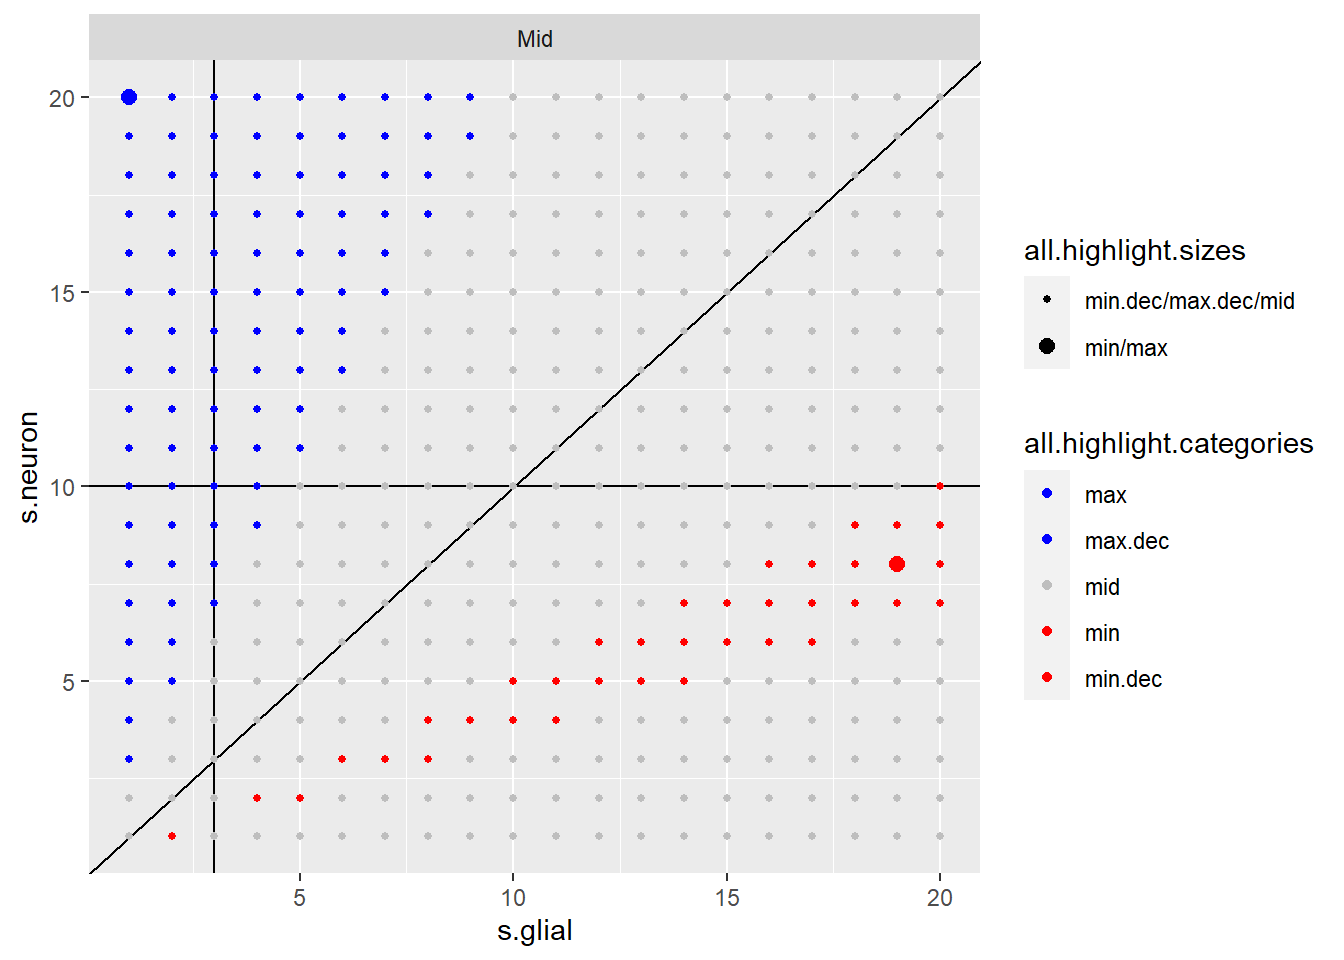
\includegraphics{pb-byblock_sopt-bias-error_k2-cohort1_files/figure-latex/unnamed-chunk-9-1.pdf}

\begin{Shaded}
\begin{Highlighting}[]
\FunctionTok{ggplot}\NormalTok{(df.res, }\FunctionTok{aes}\NormalTok{(}\AttributeTok{x =}\NormalTok{ neuron, }\AttributeTok{y =}\NormalTok{ bias.neuron.true.pred, }\AttributeTok{color =}\NormalTok{ sample.id)) }\SpecialCharTok{+} 
  \FunctionTok{theme\_bw}\NormalTok{() }\SpecialCharTok{+} \FunctionTok{geom\_smooth}\NormalTok{(}\AttributeTok{method =} \StringTok{"glm"}\NormalTok{, }\AttributeTok{se =}\NormalTok{ T) }\SpecialCharTok{+} \FunctionTok{geom\_hline}\NormalTok{(}\AttributeTok{yintercept =} \DecValTok{0}\NormalTok{)}
\end{Highlighting}
\end{Shaded}

\begin{verbatim}
## `geom_smooth()` using formula = 'y ~ x'
\end{verbatim}

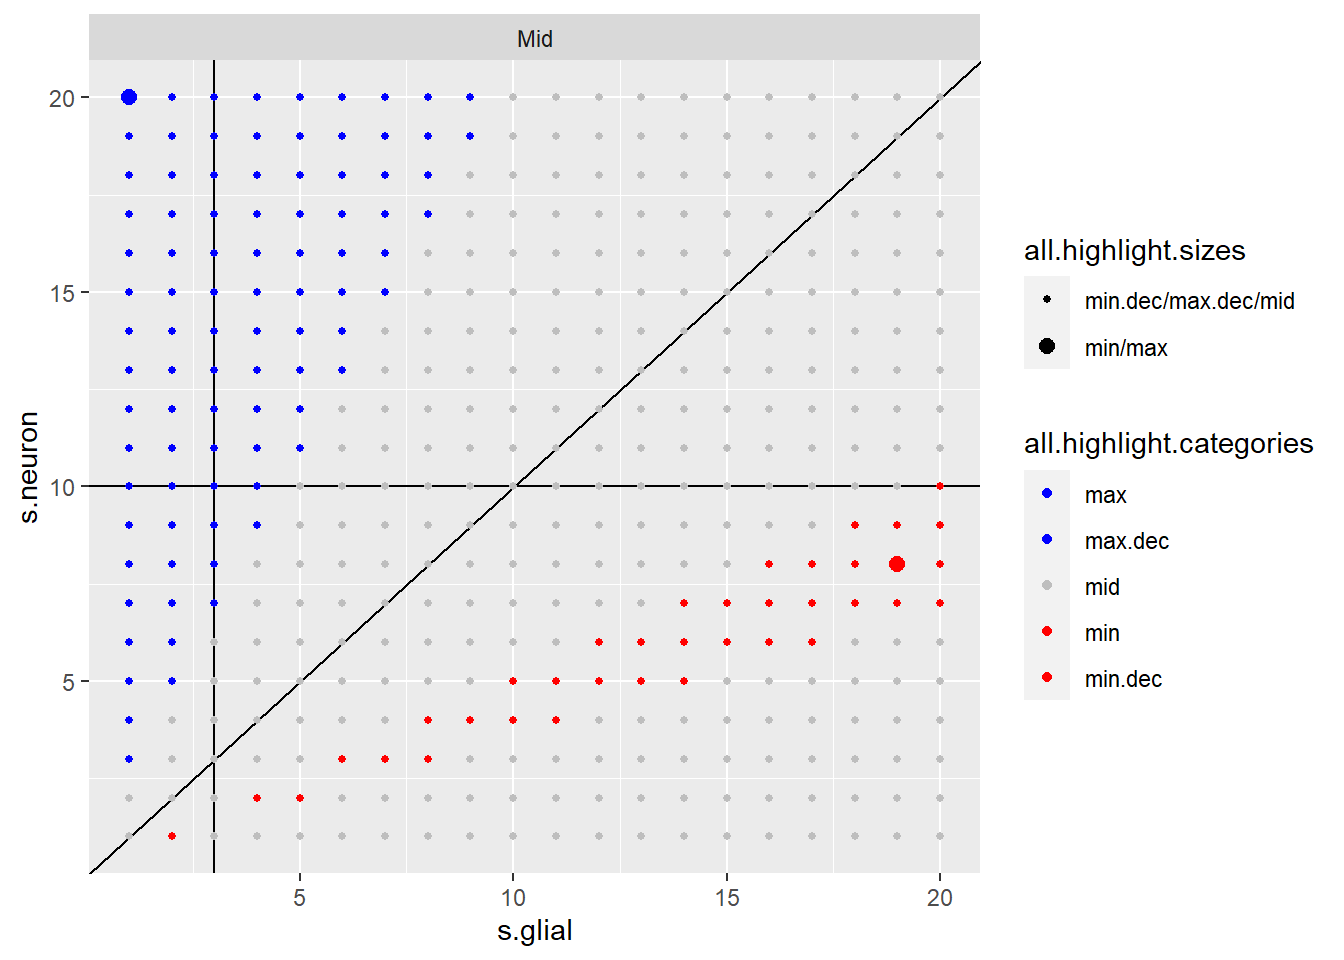
\includegraphics{pb-byblock_sopt-bias-error_k2-cohort1_files/figure-latex/unnamed-chunk-10-1.pdf}

\begin{Shaded}
\begin{Highlighting}[]
\FunctionTok{ggplot}\NormalTok{(df.res, }\FunctionTok{aes}\NormalTok{(}\AttributeTok{x =}\NormalTok{ neuron, }\AttributeTok{y =}\NormalTok{ bias.glial.true.pred, }\AttributeTok{color =}\NormalTok{ sample.id)) }\SpecialCharTok{+} 
  \FunctionTok{theme\_bw}\NormalTok{() }\SpecialCharTok{+} \FunctionTok{geom\_smooth}\NormalTok{(}\AttributeTok{method =} \StringTok{"glm"}\NormalTok{, }\AttributeTok{se =}\NormalTok{ T) }\SpecialCharTok{+} \FunctionTok{geom\_hline}\NormalTok{(}\AttributeTok{yintercept =} \DecValTok{0}\NormalTok{)}
\end{Highlighting}
\end{Shaded}

\begin{verbatim}
## `geom_smooth()` using formula = 'y ~ x'
\end{verbatim}

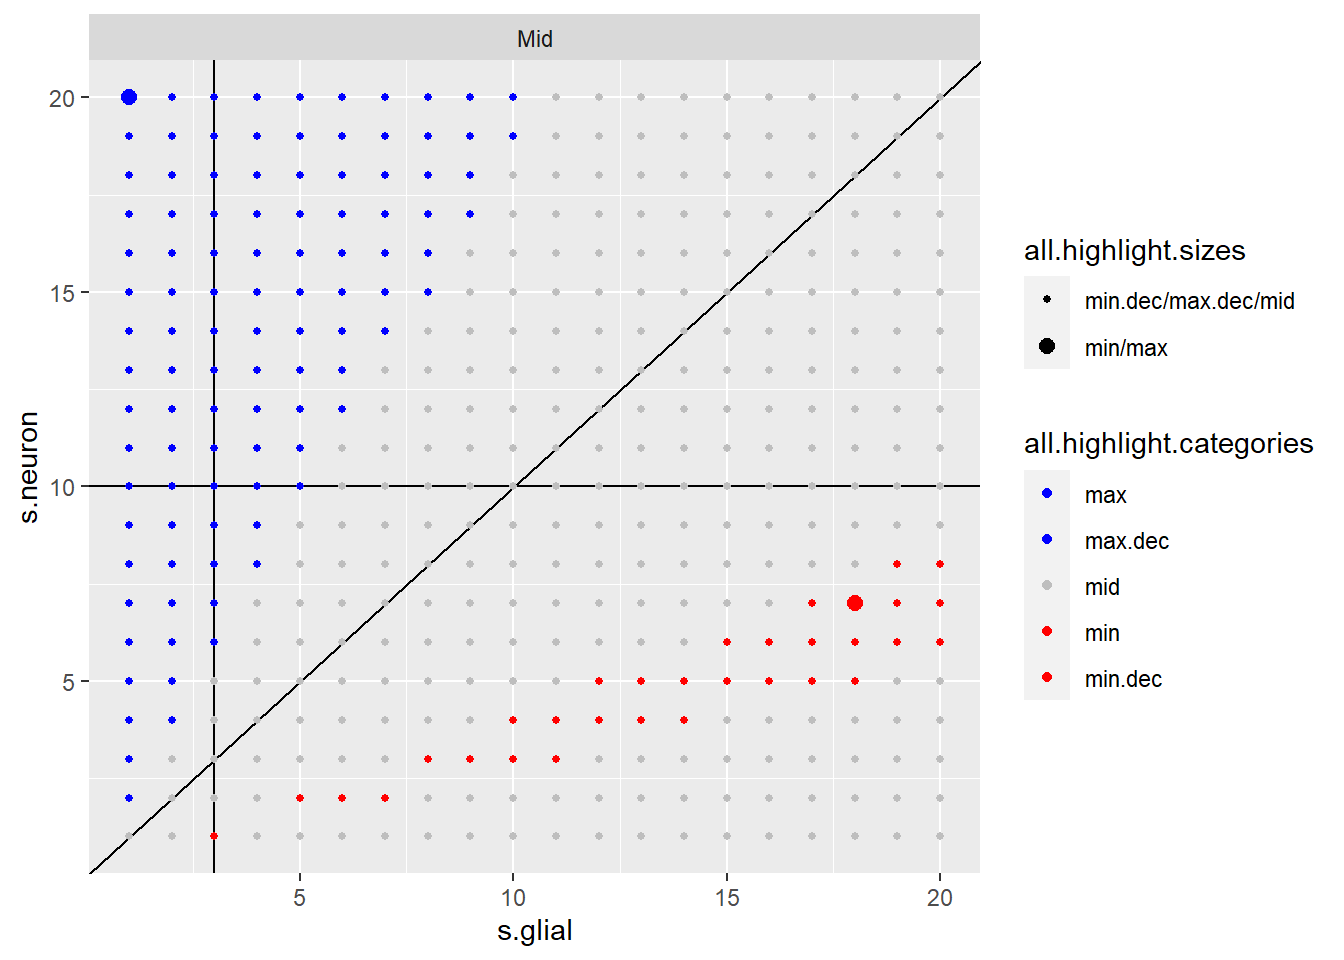
\includegraphics{pb-byblock_sopt-bias-error_k2-cohort1_files/figure-latex/unnamed-chunk-11-1.pdf}

\end{document}
